\documentclass[11pt]{article}

\usepackage[margin=2.2cm]{geometry}
\usepackage{amsmath}
\usepackage{xcolor}
\usepackage{hyperref}
\usepackage{graphicx}
\usepackage{enumitem}

\hypersetup{colorlinks=true, linkcolor=blue!50!black, urlcolor=blue!50!black}

\setlength{\parskip}{0.35em}
\setlength{\parindent}{0pt}

\title{OVMM: System Walkthrough and Approaches}
\author{}
\date{}

\begin{document}
\sloppy
\maketitle

\section*{The system in one paragraph}

A fetch command goes through one loop, repeated until the object is grasped or every
candidate location is exhausted: \emph{reason} about where the object probably is
(scene graph lookup, or an LLM guess if it isn't known) $\to$ \emph{navigate} to a
safe standoff near that location $\to$ \emph{perceive} (look, detect with SAM3,
re-aim if needed) $\to$ \emph{grasp} (AnyGrasp pose $\to$ arm joints). \texttt{core/}
is plain Python with no ROS dependency (the reasoning/planning side); \texttt{fetcher}
is the ROS 2 package that turns \texttt{core/}'s decisions into real Nav2 goals, head
trajectories, and arm motions.

\begin{center}
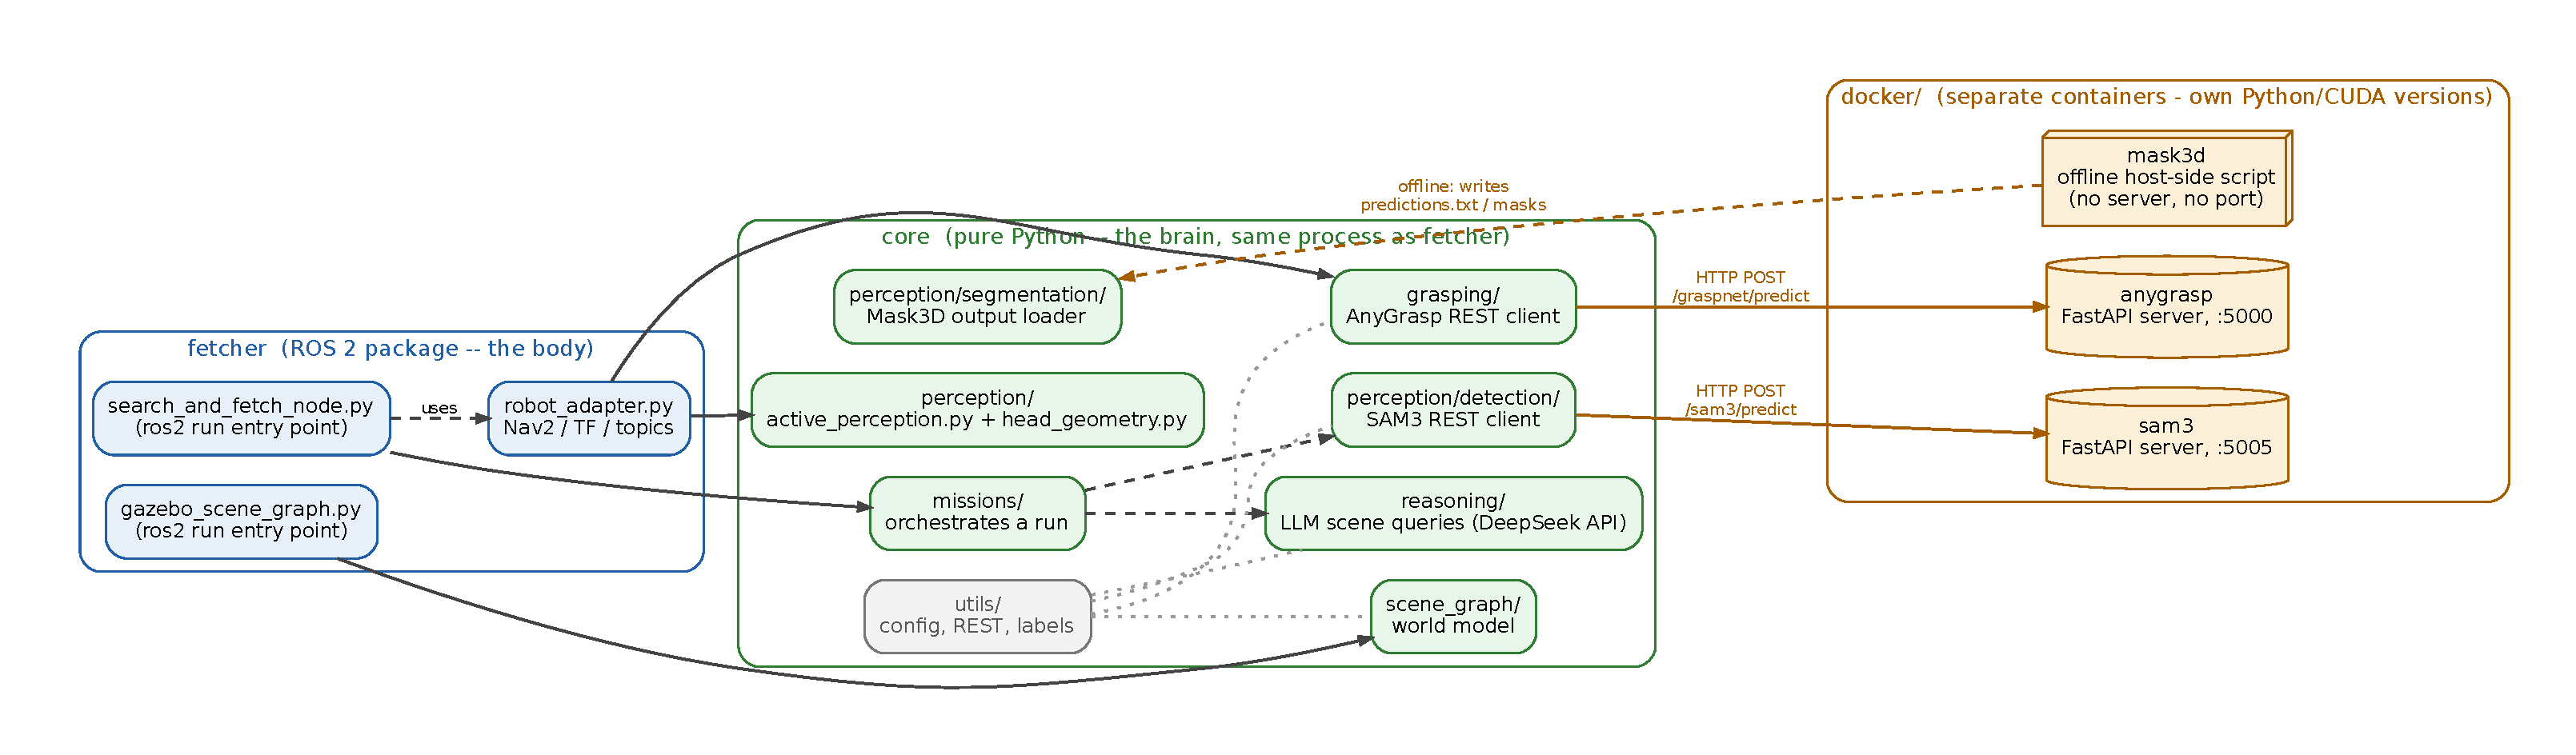
\includegraphics[width=0.6\textwidth]{architecture.pdf}
\end{center}

\section*{What each folder does}

\begin{description}[itemsep=1pt, topsep=3pt, leftmargin=1.7cm]
  \item[\texttt{perception/}] SAM3 detection client, Mask3D output loader, and the
        pure geometry for where to look/stand (\texttt{active\_perception.py},
        \texttt{head\_geometry.py}).
  \item[\texttt{scene\_graph/}] The world model: furniture/objects as nodes
        (centroid, dimensions), connected by ``sits on'' edges. Built once per scene.
  \item[\texttt{grasping/}] AnyGrasp REST client - point cloud in, ranked
        collision-aware grasp poses out.
  \item[\texttt{reasoning/}] Talks to the LLM: known-location lookup or top-$k$
        furniture prediction when the object isn't in the graph yet.
  \item[\texttt{missions/}] Orchestrates one fetch attempt end to end against a
        \texttt{RobotAdapter} protocol it never implements itself.
  \item[\texttt{utils/}] Config loading, the REST client base class, label tables.
  \item[\texttt{fetcher/}] The ROS 2 side: \texttt{robot\_adapter.py} is the only
        place Nav2/TF/topics/joint trajectories appear (it implements
        \texttt{RobotAdapter} for the HSR); the other two files are thin
        \texttt{ros2 run} entry points calling straight into \texttt{core/}.
\end{description}

\section*{Approaches}

Each of these replaced a version that looked reasonable but broke on real geometry -
the common thread is trusting live data (TF, the costmap, a fresh detection) over a
single fixed number computed once and assumed to still be true.

\textbf{World$\leftrightarrow$map frames.} The scene graph stores \texttt{world}-frame
ground truth; Nav2 plans in \texttt{map}, anchored at the robot's fixed spawn point
$t=(5.0,6.6,0)$. Every pose is converted via $p_{\text{map}} = p_{\text{world}} - t$
through a TF lookup, not assumed to already coincide.

\textbf{Reachability-aware standoff.} Instead of a fixed offset from a target,
\texttt{reachable\_approach\_pose} scans an annulus of candidate points
$(c_x + r\cos\theta_i,\, c_y + r\sin\theta_i)$ for $r\in[r_{\min},r_{\max}]$
(closest-first) against the live costmap, accepting the first point with cost
$<253$ (nav2\_costmap\_2d's inscribed-obstacle threshold). $r_{\min}/r_{\max}$ are
not fixed either: \texttt{\_reach\_band()} computes them as a clearance constant
(0.3/0.55\,m, $\approx$ the robot's footprint radius) \emph{plus} the target
furniture's own \texttt{approach\_radius} - half its \emph{shorter} horizontal
dimension, since an approach is normally perpendicular to a piece's long axis. A
small table and a long counter each get a standoff scaled to their own size.

\textbf{Height-aware look-at target.} A resting object's aim point used its
furniture's centroid $z$ - the volumetric middle of the whole piece - not where
objects actually sit. For furniture with one flat top (table/desk/coffee
table/trolley) the target is corrected to $z_{\text{top}} = c_z + h/2$. Multi-level
storage (shelf/cabinet) keeps the bulk centroid instead, since an object can be on
any internal level and the bounding-box top would aim above all of them.

\textbf{Active re-centering.} The first \texttt{look\_at} aims at the a-priori
estimate, not the object itself, so if navigation landed a bit off, that first
detection can be off-center. After it succeeds, its mask is lifted to a point cloud,
the centroid is converted back to world frame, and \texttt{look\_at} fires once more
at the object's \emph{actual} position before the final detection is used - re-sensing
instead of trusting the original estimate, with the original detection kept as a
fallback if re-detection fails.

\textbf{Nearest-of-duplicates disambiguation.} When a query matches a label that
isn't unique in the scene (two pringles cans), the LLM has no spatial awareness to
choose between them. The match is now overridden with
$\arg\min_i \lVert c_i - p_{\text{robot}}\rVert_2$ over every item sharing that label,
using the robot's live position - a geometric tie-break instead of an arbitrary
language-model one.

\textbf{Two-phase grasp motion.} Arm joints used to move together in one trajectory,
so the gripper could sweep forward while still rising - risking a clip across
whatever surface the object rests on. The arm now lifts to the target height first
with \texttt{arm\_flex\_joint} held at its retracted limit ($0.0$), \emph{then}
extends to the full target pose.

\textbf{Known limitation.} The arm-joint formula only ever uses the grasp's
\emph{position}; AnyGrasp's chosen \emph{orientation} is discarded; and
\texttt{wrist\_flex}/\texttt{arm\_roll} are fixed constants. This is the next real
fix needed, not yet attempted live - the formula is an analytic approximation, not
inverse kinematics.

\end{document}
